\subsection{Layout}
The microAmperes internal and external layout is designed to achieve an optimal balance between functionality, modularity, and serviceability. The vessel is divided into three main physical sections, consisting of the two hulls and the central watertight enclosure. Each section has a specific role in the system: propulsion and power are located in the hulls, computation and communication in the watertight enclosure, and perception sensors are distributed around the vessel. This structure simplifies cabling, improves center-of-gravity stability, and provides a clean and organized platform for integrating research equipment.
\\ \\
The port hull houses the port side battery pack and Electronic Speed Controller (ESC) that drive the left thruster, while the starboard hull contains the mirrored setup together with a Power Sense Module responsible for voltage and current monitoring. Both hulls are interconnected through a reinforced cross tube that carries power, Pulse Width Modulation (PWM), and Ethernet lines to the watertight enclosure. This cross connection ensures a robust and low latency interface between propulsion, control, and sensor systems, while maintaining mechanical symmetry and balance across the hulls.
\\ \\
On the top deck, the vessel supports a LiDAR platform and stereo camera mounts designed to provide an unobstructed 360\textdegree{} field of view. \todo{TAP: only the lidar gives 360 deg FOV} These sensors enable simultaneous environmental mapping and perception. Additional top mounted features include power switch, diagnostic status LEDs, and the antennas for GNSS, 5G, and radio communication. The overall sensor placement was chosen to ensure optimal visibility, minimal interference between radio and optical systems, and ease of access during maintenance or calibration.
\\ \\
Externally, all antennas and sensors are symmetrically arranged to guarantee signal balance and redundancy. The vessel is equipped with dual GNSS antennas mounted at the rear of each hull for precise position and heading estimation, a 5G antenna for long range communication, and a radio antenna for local telemetry. The perception suite consists of two stereo cameras and a LiDAR unit mounted on the LiDAR platform. Together, these sensors provide full 360\textdegree{} situational awareness and deliver high quality data for SLAM, obstacle detection, and perception algorithms. \todo{TAP: repetition from previous paragraph? Important to avoid repetition, also think about if all description is needed. Try to be concise and precise.}
\\ \\
The internal layout focuses on structured modularity, with all high power and propulsion related systems isolated within the hulls, and all sensitive electronics centralized in the watertight enclosure. This separation improves electromagnetic compatibility and enhances maintainability during field operations. The vessels internal wiring is routed through marine grade cable glands, organized in cable harnesses with labeled connectors for quick service and component replacement.
\\ \\
In addition, active cooling fans are installed at the rear of the hulls and inside the watertight enclosure to maintain safe operating temperatures for both computation and power electronics. Proper thermal design and airflow direction have been validated through practical testing to ensure stability under extended mission durations and high computational loads.
\begin{figure}[H]
    \centering
    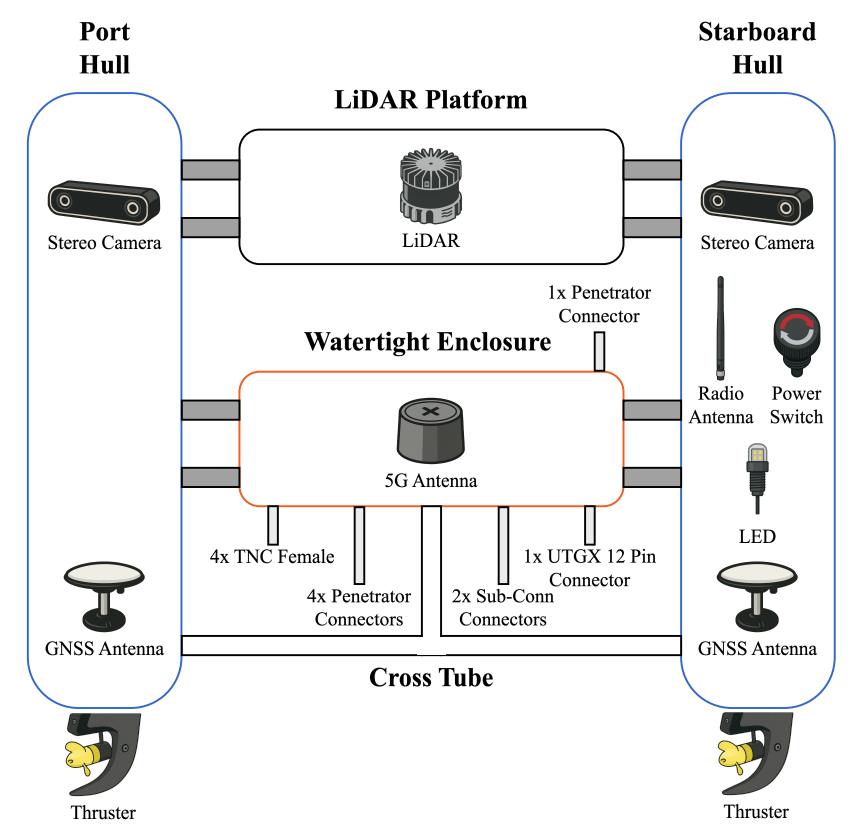
\includegraphics[width=0.7\linewidth]{Pictures/Hardware/Layout/BoatTop.png}
    \caption{Top level overview of the microAmpere vessel showing the placement of cameras, antennas, thrusters, power switches, status LEDs, and LiDAR platform. Picture taken from Luan Cao Vo Tran master thesis on microAmpere ASV.\textsuperscript{\cite{microAmpere_hardware_master_thesis1}}}
    \label{fig:microAmpere-layout-top}
\end{figure}
\begin{figure}[H]
    \centering
    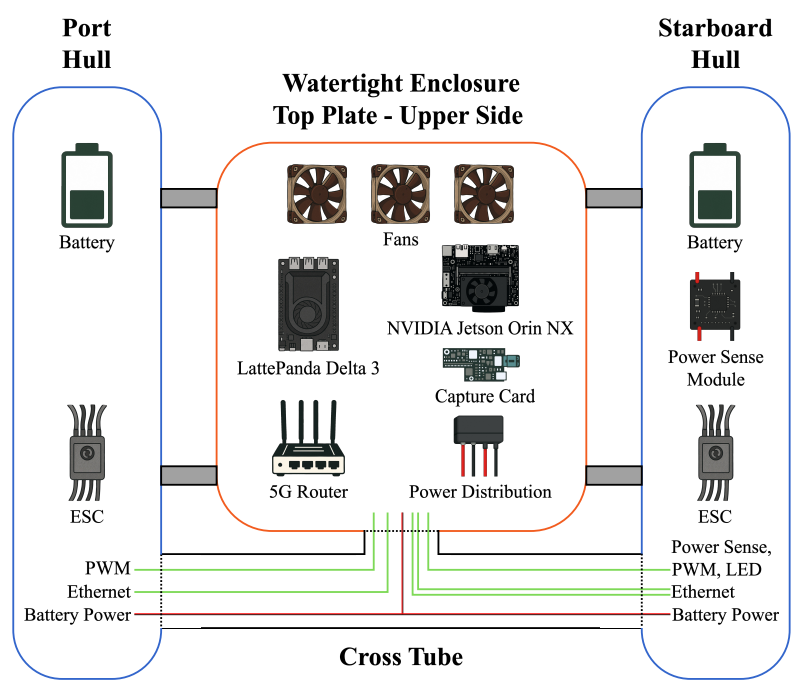
\includegraphics[width=0.7\linewidth]{Pictures/Hardware/Layout/BoatBottom.png}
    \caption{Bottom view of microAmpere showing the internal layout of batteries, ESCs, cooling fans, SBCs, capture card, and power distribution units for optimized performance and accessibility. Picture taken from Luan Cao Vo Tran master thesis on microAmpere ASV.\textsuperscript{\cite{microAmpere_hardware_master_thesis1}}}
    \label{fig:microAmpere-layout-bottom}
\end{figure}



\newpage



\noindent
Focusing on the watertight enclosure, this section contains all critical computational, power conversion, and synchronization electronics of the microAmpere system. The internal structure follows a two layer plexiglass mounting design with a top and bottom plate. This setup maximizes thermal efficiency, ensures proper airflow, and allows easy access for maintenance or hardware upgrades.
\\ \\
The top plate upper side holds the main compute stack, including the \textit{``NVIDIA Jetson Orin NX''}, \textit{``LattePanda 3 Delta''}, and the \textit{``Teltonika RUTX50 5G router''}. These components are mounted alongside a power distribution module and a set of \textit{``Noctua 60 mm cooling fans''} for optimal airflow and thermal stability during intensive computational loads. The placement of these units also provides clear cable routing paths and short communication links between processing and networking hardware.
\\ \\
The underside of the top plate contains the \textit{``DC/DC converters''} rated at 30 W and 150 W, a \textit{``fuse board''}, and the fan bracket assembly. These converters supply stable 12 V and 5 V lines to different subsystems including the compute boards, router, Sentiboard, and auxiliary electronics. The components are arranged for efficient heat dissipation and quick replacement in case of hardware maintenance.
\\ \\
The bottom plate top side integrates the primary navigation and synchronization modules. It includes the \textit{``Xsens MTi-680G IMU''}, dual \textit{``u-blox ZED-F9P GNSS receivers''}, and the custom \textit{``Sentiboard''} used for precise hardware timestamping and signal synchronization. The stacked layout minimizes wiring complexity, reduces signal interference, and maintains clear access for diagnostics and firmware updates.
\\ \\
Overall, the watertight enclosure layout emphasizes modularity, cooling efficiency, and reliability. By separating compute, power, and navigation layers, the design reduces thermal coupling between components and improves system robustness during long duration field operations. This configuration allows the microAmpere to operate safely under variable weather and computational conditions while maintaining high data integrity across all subsystems.
\begin{figure}[H]
    \centering
    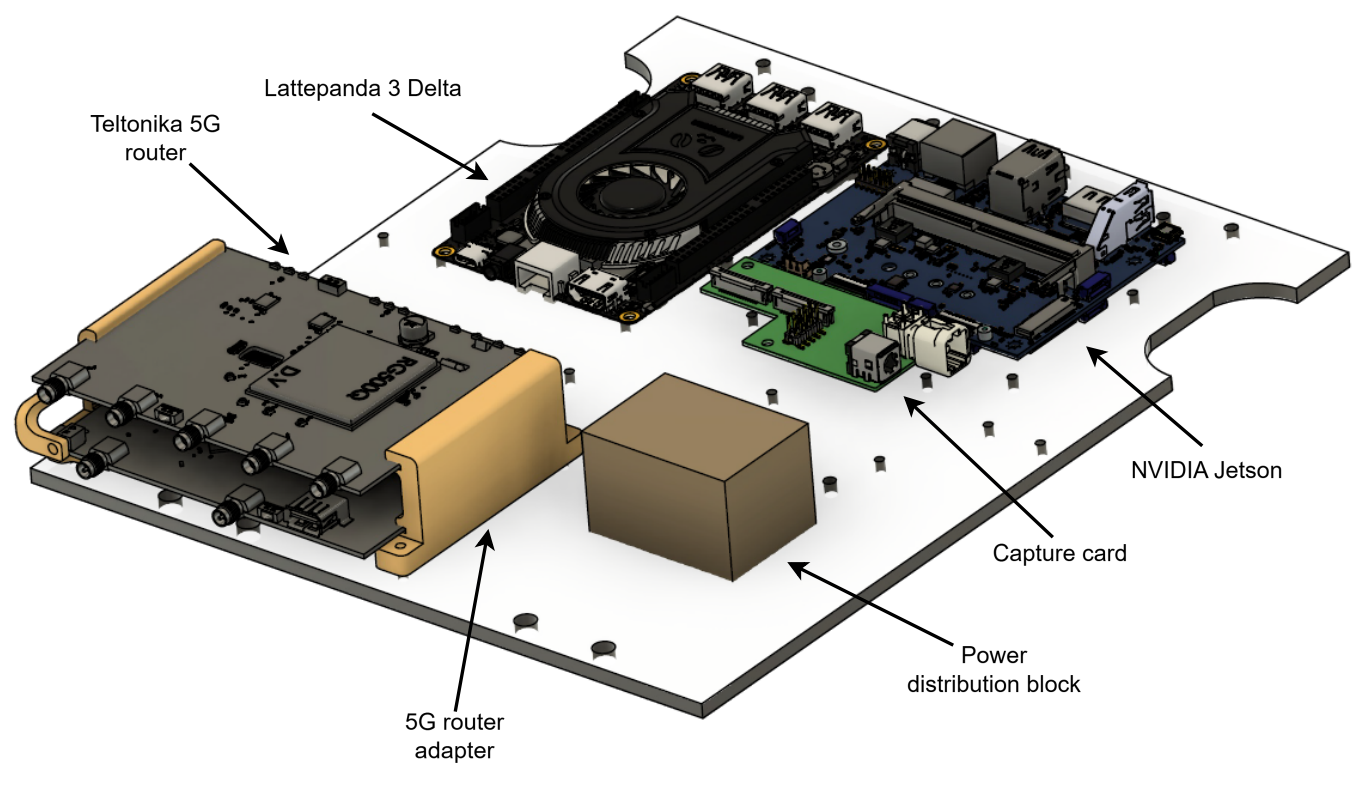
\includegraphics[width=0.9\linewidth]{Pictures/Hardware/Layout/BoxTopPlateTop.png}
    \caption{Watertight enclosure top plate (upper side) showing the main compute stack with Jetson Orin NX, LattePanda 3 Delta, and Teltonika RUTX50 router. Picture taken from Henrik Reimers master thesis on microAmpere ASV.\textsuperscript{\cite{microAmpere_hardware_master_thesis1}}}
    \label{fig:microAmpere-layout-topplate-top}
\end{figure}
\begin{figure}[H]
    \centering
    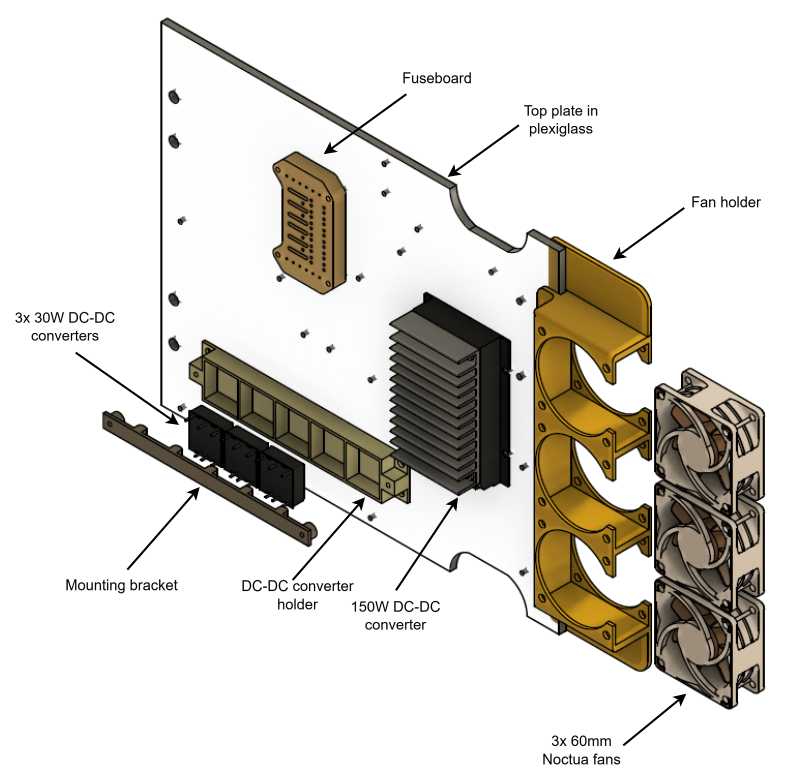
\includegraphics[width=0.8\linewidth]{Pictures/Hardware/Layout/BoxTopPlateBottom.png}
    \caption{Underside of the top plate showing the DC/DC converters, fuse board, and cooling fans for power regulation and heat management. Picture taken from Henrik Reimers master thesis on microAmpere ASV.\textsuperscript{\cite{microAmpere_hardware_master_thesis1}}}
    \label{fig:microAmpere-layout-topplate-bottom}
\end{figure}
\begin{figure}[H]
    \centering
    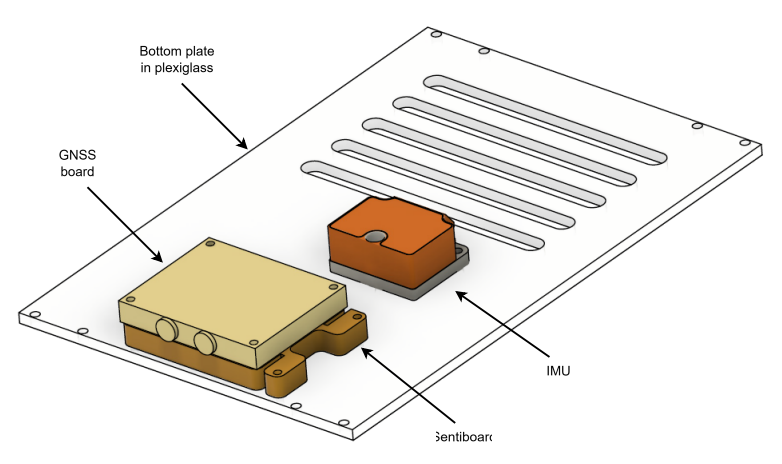
\includegraphics[width=0.8\linewidth]{Pictures/Hardware/Layout/BoxBottomPlateTop.png}
    \caption{Bottom plate layout containing the IMU, Sentiboard, and GNSS receivers used for precise navigation and time synchronization. Picture taken from Henrik Reimers master thesis on microAmpere ASV.\textsuperscript{\cite{microAmpere_hardware_master_thesis1}}}
    \label{fig:microAmpere-layout-bottomplate}
\end{figure}
